\chapter{Introduction}\label{chap:introduction}

\begin{comment}
Andreas
1.1 Domain . . . . . . . . . . . .
1.2 Existing Solutions . . . . . . 
1.3 Task Description . . . . . . . 
1.4 Project Goals . . . . . . . . .
1.4.1 Effect Goals . . . . . . . . 
1.4.2 Result Goals . . . . . . . . 
1.4.3 Learning Goals . . . . . . . 
1.5 Framework . . . . . . . . . . .
1.6 Project Constraints
1.7 Group Background
1.8 Project organization
1.8.1 Responsibilities and roles
1.9 Target Audience 
1.10 Report 
1.10.1 Structure 
\end{comment}

\begin{comment}
sander
1.1 Problem definition . . . . . . .
1.2 Scope of work. . . . . . . . . .
1.3 Requirements and constraints . .
1.4 Goals. . . . . . . . . . . . . . 
1.5 Approach . . . . . . . . . . . .
1.6 Group background and motivation 
1.7 Thesis structure .

Effektmål = Business goal (evt Impact)
Rammer = Framework (føringer fra oppdragsgiver)
Omfang = Scope
Problemområde = Problem area
Begrensninger = Limitations (utenfor din kontroll)
Avgrensninger = Delimitations (noe du bestemmer)
Oppgavedefinisjon = Problem statement ("tese")
\end{comment}

The forestry industry is essential to sustainable resource management, environmental conservation, and economic development. Effective forest management requires expertise in areas such as forest operations and infrastructure maintenance. To support these efforts, various organizations play a key role in sharing knowledge and providing professional training to uphold best practices.

One such organization is Skogkurs\footnote{\url{https://skogkurs.no/}}, a non-governmental organization established in 1958. The institute operates as a partnership, with 36 forestry organizations and scientific institutions as its members. Its activities are nationwide and encompass a wide range of topics, including forest management, the construction and maintenance of forest roads, as well as forestry operations and technical practices \cite{skogkurs_eng}. Through its initiatives, Skogkurs aims to enhance the competence of professionals within the forestry industry and to promote knowledge of forests and nature to schools and the general public \cite{skogkurs_nor}. 

\section{Problem Definition}
% Legge til en figur? Evt. fra denne: https://nibio.brage.unit.no/nibio-xmlui/bitstream/handle/11250/3037571/NIBIO_RAPPORT_2022_8_147.pdf?sequence=1
The Nordic forestry industry faces increasing challenges in ensuring stable timber transport throughout the year. Changes in climate have extended the snow-free season, creating variability in forest road conditions due to shifts between frozen, dry, and rainy periods. Addressing these challenges requires digital tools that can assess which forest roads are accessible during different weather conditions. A schematic illustration of forest road conditions is shown in \autoref{fig:yearlytimeline}.

\begin{figure}[h]
    \centering
    \centerline{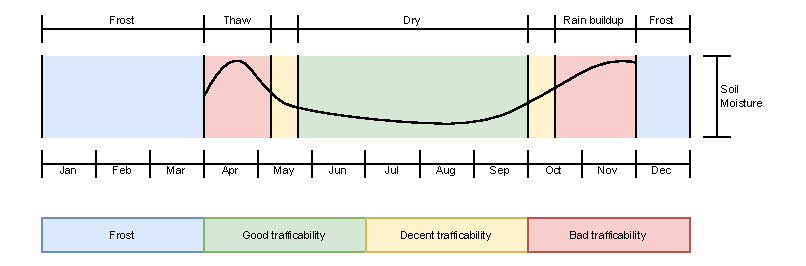
\includegraphics[width=1.3\linewidth]{figures/yearlytimeline.pdf}}
    \caption{Schematic illustration of trafficability and soil moisture throughout the year}
    \label{fig:yearlytimeline}
\end{figure}

Recent research has focused on developing methodologies for digitally classifying forest road load-bearing capacities based on soil types and weather conditions. For example, a nationwide pilot study demonstrated that soil types, such as well-drained materials like \gls{glaciofluvial deposit}s, are more suitable for year-round use, while finer sediments require specific conditions like frost or dry periods. A plot showing different soil types' load-bearing capacity dependent on the amount of water in the soil is shown in \autoref{fig:load_to_drought_graph}. These findings support the potential for fully digital solutions to predict road accessibility based on a combination of weather patterns and road construction characteristics \cite{fjeld2023trafficability}.

\begin{figure}[h]
    \centering
    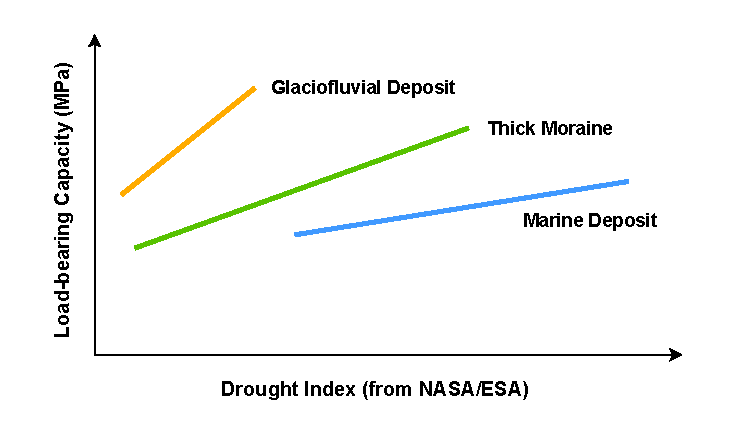
\includegraphics[width=0.7\linewidth]{figures/bæreevne_tørkeindex.pdf}
    \caption[Graph comparing load-bearing capacity to drought index]{Graph comparing load-bearing capacity to drought index, recreated from the task description [\hyperref[appendix:task_description]{Appendix \ref*{appendix:task_description}}]}
    \label{fig:load_to_drought_graph}
\end{figure}

While these studies highlight the feasibility of digital road classification, practical solutions for transport managers remain limited. Current industry practices often rely on experience-based assessments and manual planning, leading to inefficiencies and uncertainty. Although some digital tools have been developed to assist in forestry road trafficability assessment, they are not universally applicable across different regions. This thesis introduces a prototype system designed to address these challenges by combining environmental data, forecasting, and intuitive map-based visualization to support more informed and proactive decision-making.

\section{Existing Solutions}

One example is Harvester Seasons\footnote{\url{https://harvesterseasons.com/}}, developed by the Finnish Forest Center, which provides weekly forecasts of road conditions based on soil moisture, temperature, and snow depth. These forecasts use data from sources like \acrshort{nasa}'s \gls{smap} and \acrshort{esa}'s \Gls{sentinel-1} satellites to generate relative load-bearing predictions for winter and snow-free seasons [\hyperref[appendix:task_description]{Appendix \ref*{appendix:task_description}}]. While this tool offers valuable insights, it is limited to Finland and does not provide road condition data for Norway. As a result, it does not meet the needs of Skogkurs, which requires a solution tailored to Norwegian forest roads. This highlights the gap in available tools and the need for a localized approach that accounts for Norway's specific terrain, climate, and forestry infrastructure.

The current process of scheduling operations for transport managers is based on weather conditions and road \gls{trafficability}, responding either to constraints (e.g., wet conditions) or taking advantage of favorable circumstances (e.g., dry periods). These decisions rely on factors such as seasonal temperature trends, regional precipitation, and local experience. Surface deposits and their \gls{permeability} also affect transport timing and road usability, with adverse weather and poor road \gls{trafficability} posing significant challenges to wood supply and transport logistics \cite[p.~2]{fjeld2023trafficability}. The primary tool used for managing these logistics is VSYS Transport, developed by Skogdata\footnote{\url{https://www.skogdata.no/digitale-produkter}}. VSYS supports forestry logistics by offering functionalities for transport order management, route planning, assignment tracking, deviation handling, freight documentation, and settlement processing for carriers, but lacks features for easily assessing road trafficability \cite{skogdata2024vsys}.

\section{Framework}

\textcolor{orange}{NOE TEKST}

\section{Project Organization}

\textcolor{orange}{NOE TEKST}

\section{Thesis Structure}

\begin{comment}
    Fra salamander:
    This thesis includes a list of acronyms and a glossary, which can be found above the introduction. We were provided with a LaTeX template from NTNU [13], made by Ivar Farup, and followed this as it is a baseline for computer science theses. In addition to the chapters the template suggested, we added a couple of additional ones: Chapter 3 Development Plan and Chapter 6 Graphical User Interface. Below is a listing of all chapters featured in this thesis, in chronological order

    For oss:
    Ikke Ivar, men CoPScE@NTNU (?), template
\end{comment}

This thesis uses a template by CoPCSE@NTNU\footnote{\url{https://github.com/COPCSE-NTNU/thesis-NTNU}} blabla added \autoref{chap:mapdatasources} (Map Data Sources) due to its importance in the project.

\begin{enumerate}
    \item \textbf{\hyperref[chap:introduction]{Introduction}:}
    \item \textbf{\hyperref[chap:requirements]{Requirements}:}
    \item \textbf{\hyperref[chap:technicaldesign]{Technical Design}:}
    \item \textbf{\hyperref[chap:mapdatasources]{Map Data Sources}:}
    \item \textbf{\hyperref[chap:developmentprocess]{Development Process}:}
    \item \textbf{\hyperref[chap:implementation]{Implementation}:}
    \item \textbf{\hyperref[chap:deployment]{Deployment}:}
    \item \textbf{\hyperref[chap:qualityassuranceanduserfeedback]{Quality Assurance and User Feedback}:}
    \item \textbf{\hyperref[chap:discussion]{Discussion}:}
    \item \textbf{\hyperref[chap:conclusion]{Conclusion}:}
\end{enumerate}

